\chapter{Running \maken{} in Context}
\label{chap:context}

In the previous chapter we presented some toy examples. However, in real neuroimaging life one deals with hundreds of subjects with multiple types of scans and many planned analyses. To keep this straight requires some conventions, whether you use \maken{} or not. Here we describe some conventions that are useful for managing realistic projects.

\section{File Naming Conventions}
\label{sec:naming}

File naming conventions are critical for scripting in general, and for Makefiles in particular. \maken{} is specifically designed to turn files with one extension (the extension is the last several characters of the filename) into files with another extension. For example, in \autoref{make:recipe1} we turned a file with an extension ``T1.nii.gz'' into a file with the extension ``T1_skstrip.nii.gz.'' 
\mymarginnote{!}{``\textbf{Extension}'' often refers to the file suffix, e.g., ``.csv,'' but there is no reason it must be limited to a fixed number of characters after a period.}

So we can use naming conventions within a project, and across projects consistently to reuse rules that we write for common operations. In fact, \maken{} has many built-in rules for compiling programs that are absolutely useless to us. But we can write our own rules.

Thus, it is important to decide upon naming conventions. 

\subsection{Subject Identifiers}

The first element of naming conventions is the subject identifier. This is usually the first part of any file name that we might end up using outside of its directory. For example, we might include the subject identifier in the final preprocessed resting state data, allowing us to dump all those files into a new directory for subsequent analysis with another program, without having to rename them or risk overwriting other subject files. Some features (by no means exhaustive) that may be useful for subject identifiers are:

\begin{easylist}[enumerate]
	& \textbf{They should contain some indicator of which project the subjects belong to.} \\
	This is particularly important if you work on multiple projects, or if you may be pooling data from multiple studies. Typically choose a multi-letter code that is the prefix to the subject ID.
	& \textbf{If applicable, they should contain some indicator of treatment group that the subject belongs to.} \\
	It is helpful to indicate in the subject ID (usually with another letter or digit code) whether the subject is part of a treatment group or a control.
	& \textbf{They should be short.} \\
	Short names are easier to type and to remember, and make it easier to work with lists of directories that are named according to the subject id.
	& \textbf{They should be the same length.} \\
	This is not necessary but helpful for pattern matching using wildcards in a variety of contexts within \maken{} and without.
	& \textbf{They should sort reasonably in UNIX.} \\
	Many utilities ultimately require a list of filenames, which is easy to generate using wildcards and the treatment group code if the subject ID sort order is reasonable. The classic problem is to name subjects S1 \ldots S10, S11 -- the subjects will not be in numeric order without zero-padding to the subject numbers.
	& \textbf{They should be easy to type.} \\
	\bashn{} has many tricks to help you avoid typing, but when you have to type, the farther you have to move the longer it takes. Do you really need capital letters? 
	& \textbf{They should be easy to remember for short periods of time.} \\
	My attention span is very short when doing repetitive tasks; subject IDs that are nine-digit random numbers are harder to remember than subject IDs that are four letter random sequences. 
	& \textbf{They should be easy to divide into groups using patterns.} \\
	My favorite set of subject IDs were randomly generated four letter sequences that sounded like fake English words, making it easy to divide the subjects into groups of just about any size using the first letters and wildcards. This makes it very easy to test something on a subset of subjects. 
	& \textbf{They should be consistently used in all data sets within the project.} \\
	If the subject identifier is ``RC4101'' in a directory, it should not be ``RC4-101'' in the corresponding REDCap database\footnote{REDCap is the Research Electronic Data Capture web application that we use for storing subject-specific information.} and ``101'' in the neuropsychological data. It is easier if everyone can decide upon one form of name.
\end{easylist}

\subsection{Filenames}

File naming conventions begin with converted raw data (NIfTI files derived from the original DICOMs, for example), and continue on for each level of processing. We find it helpful to give these files specific names and then to perform subject-specific processing within the subject/session directory. The filenames for a recent active project are shown in \autoref{table:filenames}, where the subject ID is ``RTI001.''

\rowcolors*{2}{gray!50}{white} 	% alternating row coloing, starting on row 2 (ignore header)
\def\arraystretch{1.2}	% with all the caps, this table gets a little crammed. 
\begin{figure}[h!]
	\begin{tabularx}{\linewidth}{ >\ttfamily l X } % >\ttfamily applies monospaced font to column 1
											% column 1 expands, and forces 2 to shrink and wrap
		\rowcolor{gray!75}
		\normalfont\textbf{Filename} 		& \textbf{Description} 	\\ \hline
		RTI001_T1_brain.nii.gz				& Skull stripped T1 MPRAGE image 	\\  
		RTI001_T1.nii.gz					& T1 MPRAGE image 					\\  
		RTI001_read.nii.gz					& Reading task scan 				\\  
		RTI001_read_rest.nii.gz				& Resting state scan for reading session	\\ 
		RTI001_read_fMRIB0_phase.nii.gz		& $B_0$ Field map phase image for reading session\\
		RTI001_read_fMRIB0_mag.nii.gz		& $B_0$ Field map magnitude image for reading session\\  
		RTI001_read_fMRIB0_mag_brain.nii.gz & Skull stripped $B_0$  magnitude image \\  
		RTI001_write.nii.gz					& Writing task scan 				\\  
		RTI001_write_rest.nii.gz			& Resting state scan for writing session	\\  
		RTI001_write_fMRIB0_phase.nii.gz	& $B_0$ Field map phase image for writing session\\
		RTI001_write_fMRIB0_mag.nii.gz		& $B_0$ Field map magnitude image for writing session\\  
		RTI001_write_fMRIB0_mag_brain.nii.gz	& Skull stripped $B_0$ magnitude image	\\ 
		RTI001_DTI.nii.gz					& DTI image 						\\ 
		bvecs.txt							& b-vectors for  DTI processing 	\\
		bvals.txt 							& b-values for DTI processing\\ \hline
	\end{tabularx}
	\caption{Example of good file naming conventions}
	\label{table:filenames}
\end{figure}

The specific file names chosen are not as important as consistency in the use of extensions and names, and documentation of what these files are and how they were processed. The more you can keep things the same between projects, the more Makefiles you will be able to reuse from one study to another with minimal changes. 

\section{Directory Structure}
\label{sec:dir}

Typically, we create a directory for each project. Within that project directory is storage for scripts, masks, data files from other sources (e.g., cognitive or neuropsychological data) and subject neuroimaging data. Subjects may have different timepoints or occasions of imaging data, as well as physiological data and task-related behavioral data.
An example hierarchy (for project Udall) is shown in \autoref{figure:udalldir}. We have recreated this directory structure in \texttt{\$MAKEPIPELINES/Udall}, without any actual MRI data, so that you can follow the structure. You can also look at \autoref{sec:practicum2} for a description of how to set up a similar directory structure for an actual data set.

\begin{center}
	\begin{figure}[h!]
		\dirtree{%
			.1 /project_space/Udall.
			.2 bin\DTcomment{Holds \bashn{} scripts written for this project}.
			.3 R\DTcomment{Holds R scripts}.
			.3 tcl\DTcomment{Holds tcl scripts}.
			.2 data\DTcomment{Other sources of data for all subjects}.
			.2 lib\DTcomment{Holds things that are used by many scripts and analyses}.
			.3 makefiles\DTcomment{Makefiles for this project}.
			.3 networkROIs\DTcomment{A set of ROI masks for fMRI analysis}.
			.3 tractographyMasks\DTcomment{A set of masks for tractography analysis}.
			.2 freesurfer\DTcomment{Freesurfer (cortical thickness) runs}.
			.2 tbss\DTcomment{Group-level Tract-Based Spatial Statistics analyses}.
			.2 subjects\DTcomment{All subject data collected in neuroimaging sessions}.
			.3 SUBJECT\DTcomment{A specific subject}.
			.4 session1\DTcomment{Difference subject sessions}.
			.4 session2.
			.4 session3.
			.5 behavioral\DTcomment{Subject behavioral (e.g., task) data}.
			.5 Dicoms\DTcomment{Original dicoms}.
			.5 Parrecs\DTcomment{PAR/REC files, the native Philips scanner format}.
			.5 physio\DTcomment{Physiological data}.
			.5 xfm_dir\DTcomment{Registration files}.
			.3 session3/SUBJECT\DTcomment{Symbolic link to the subject/session3 directories}.
			.3 incoming\DTcomment{Zip files with subject data from the scanner.}.
		}
		\caption{An example of a project directory.}
		\label{figure:udalldir}
	\end{figure}
\end{center}

This directory is typically protected so that only members of the project who are permitted by the Institutional Review Board to access the data may \texttt{cd} into the directory, using a specific group related to the project. The setgid bit \mymarginnote{?}{The \texttt{setgid} bit on a directory ensures that files created here assume the group to which the directory belongs, and not the group to which the person creating them belongs.} is set on the project directory and the file permissions are set by default to permit group read, write, and execute permission for each individual so that files people create within the directory substructure are accessible by others in the project. 


The structure is set up for a longitudinal project, where each subject is imaged at separate time points (sessions). All subject data is stored under the directory subjects (under subdirectories corresponding to each session). However, because often it is convenient to conduct analyses on a single time point, we create a convenience directory at the top level (e.g., session3) which has symbolic links to all of the subjects' session 3 data. This can make it easier to perform subject-specific processing.

Notice that in the project directory, we keep scripts that we write to process the data in the \texttt{bin} directory. Although \texttt{bin} historically is where ``binary'' executable files are kept, the distinction between executable \bashn{} scripts and compiled executables is not terribly important. In this example we separate \texttt{tcl} scripts and \texttt{R} scripts to make things neater. 

Other data files and miscellaneous support files for workflow are stored in the \texttt{lib/} subdirectory. Again, your naming conventions may differ and there may be more categories than we have, but it is important to decide upon some structure that everyone agrees upon for the project. This makes it much easier to find things.

We find it useful to locate the results of some subject-specific processing (e.g. co-registration of files, subject-level DTI processing, subject-level task fMRI processing) in the subject/session directories. However, other types of single-subject (and group) analyses are more conveniently performed in directories (e.g. \texttt{freesurfer/}, \texttt{tbss/}) that are stored at the top level of the project.

Data files that are collected from non-neuroimaging sources are usually kept in text (tab or comma-separated) form in the \texttt{data/} directory so that scripts can find and use them (e.g., to use the subject age or some cognitive variable as a regressor in an analysis). We have found it very useful to document, manage, and merge this data very carefully, including the important QA variables that describe whether or not a subject's scan should be included in analyses.

Finally, note that we have a directory labeled \texttt{incoming}. This is a scratch directory (it could be a symbolic link to a scratch drive) for placing zip files that come from the scanner, that contain the dicoms for the scan, the Philips-specific PAR/REC files, the physiological data logged (used to correct functional MRI data for heart rate and respiration-related signal) and data from scanner tasks (e.g., EPRIME files).

\section{Setting up an Analysis Directory}
\label{sec:analysisdir}

Up until this point we have only seen little examples of makefiles that process subjects within a single directory. However, real studies include many subjects and many analyses; each analysis often produces hundreds of files per subject. Often, several researchers are trying to conduct different analyses on the same data set at the same time.

% add reference to incoming makefile
For these reasons, we use a collection of makefiles to manage a project. This section describes this basic recipe (which is a little complicated). You can also see this recipe implemented in \texttt{Udall}. Typically the steps involving creating subject directories and links are done by a script or an ``incoming'' makefile at the time that the subject data appears from the scanner. Better, if you use an archival system that you can write programs to access (for example, XNAT) a script can create all the links and name files nicely for you (see \nameref{chap:XNAT}). %%% Note this is Karl's example

This recipe relies on the concept of a ``symbolic link.'' This is a file that points to another file or directory. A symbolic link allows you to access a file or directory using a different pathname. If you remove the link, you will not remove the thing that it points to. However, if you remove the target of the link, the link won't work any more. 

To create a symbolic link, use the \texttt{ln} command.
\bashcmd{ln -s target linkname}

\texttt{target} is the path of the file you're linking to, and \texttt{linkname} is the name of the new symbolic link.

Target paths can either be absolute or relative, but they must be relative to their new location (in \texttt{linkname}). For example, using the directory structure in \autoref{figure:udalldir}, the command to create the link \texttt{session1/RC4101} would look like this (run from \texttt{Udall/session1}:
\bashcmd{ln -s ../subjects/RC4101/session1 RC4101}


\subsection{Defining the basic directory structure}
Let us assume the project home (\texttt{PROJHOME}) is called \texttt{\$MAKEPIPELINES/Udall/}. There are three scans per individual. Let us also assume there are two subjects: RC4101 and RC4103. These are the directories that need to be in place. Note we organize the actual files by subject ID and scan session. However, to make processing at each cross-sectional point easier, we create directories with symbolic links to the correct subject/session directories. This flexibility helps in many ways to make cross-sectional and longitudinal analyses easier.

All simple subject-specific processing is well-organized within the subject/session directories (for example, skull-stripping, possibly first level FEAT, DTI analysis, co-registrations). We normally run FreeSurfer in a separate directory, because it likes to put directories in a single place. Analyses that combine data across subjects or timepoints (e.g. TBSS) best go in separate directories.

\autoref{figure:longdirtree} shows an example directory for a longitudinal study.

\begin{center}
	\begin{figure}
		\dirtree{%
			.1 /project_space/Udall.
			.2 subjects\DTcomment{All subject data collected in neuroimaging sessions}.
			.3 RC4101.
			.4 session1.\DTcomment{Subject-level processing happens here.}.
			.4 session2.
			.4 session3.
			.3 RC4103.
			.4 session1.
			.4 session2.
			.4 session3.
			.2 session1/RC4103\DTcomment{Symbolic link to subjects/RC4103/session1.}.
			.2 session2/RC4101\DTcomment{Symbolic link to subjects/RC4101/session2.}.
			.2 session2/RC4103\DTcomment{and so on.}.
			.2 session3/RC4101.
			.2 session3/RC4103.
		}
	\caption{A longitudinal analysis directory.}
	\label{figure:longdirtree}
	\end{figure}
\end{center}

\subsection{Creating the session-level makefiles}
We will do all the subject-level processing from the \texttt{PROJHOME/sessionN/} directories. You will need to create a Makefile in \texttt{PROJHOME/session1}, \texttt{PROJHOME/session2}, and \texttt{PROJHOME/session3} whose only purpose is to run \maken{} within all the subject-level directories beneath it.  
\autoref{make:seshlevel} shows the example session-level makefile (\texttt{Udall/subjects/makefile_session.mk}).

\mymarginnote{?}{\textbf{\mypound}: the \maken{} comment character.}

\begin{make}{Session-level Makefile}{make:seshlevel}
	\# Top level makefile \\
	\# make all will recursively make specified targets in each subject directory.\\
	
	SUBJECTS=\$(wildcard RC4???) \\
	
	\maker{.PHONY}{all \$(SUBJECTS)} \\

	
	\maker{all}{\$(SUBJECTS)} \\
	
	\maker{\$(SUBJECTS)}{} \\
	\tab \$(MAKE) --directory=\$@ \$(TARGET)  \\
	
\end{make}

This Makefile obtains the list of subjects using a wildcard (so it expects to be in a directory where each subject has its own subdirectory). We will create symbolic links to this Makefile later.

The name of the subject directory is declared to be a phony target, so even if it exists, \maken{} will try to rebuild it. The recipe to do this is the very last line, which calls \maken{} recursively within each subject directory. It also passes along a \texttt{TARGET} variable. If unspecified, this would be the first target in the subject specific makefile.

\subsection{Creating the common subject-level makefile for each session}
As we described, the session-level makefile only exists to call \maken{} within all the subdirectories (symbolic links) in each session. So, we need to create a makefile within each subdirectory. However, we expect that the only thing that is different about each session is session-specific processing, which can be controlled by a \texttt{SESSION} variable. We can create a single subject-specific makefile and set up symbolic links to it just like we intend to do with the session-level makefile. \autoref{make:subjlevel} is an example of a subject-level makefile that can be seen at \texttt{Udall/subjects/makefile_subject.mk}.

\begin{make}{Subject-level makefile}{make:subjlevel}
        SESSION=\$(shell pwd|egrep -o 'session[0-9]'|egrep -o '[0-9]')\\

        subject=\$(shell pwd|egrep -o 'RC4[0-9][0-9][0-9]')\\
        \maker{test}{}\\
	         \tab @echo Testing that we are making \$(subject) from session \$(SESSION)\\

\end{make}

The subject-level makefile defines critical variables, such as the \texttt{SESSION}, which it obtains from the directory path, and the \texttt{subject} variable, which it also obtains from the directory path and a regular expression that matches the expected subject name. To set these variables we use the program \texttt{egrep}, which allows us to extract a specific pattern from the current working directory.

The only rule is a little dummy rule (because we have no actual data in this test directory) that ensures we have set these variables directly. 

\subsection{Creating links to the session-level makefile}
Recall that the session-level makefile needs to be located within the directories \texttt{Udall/session1},\texttt{Udall/session2} and \texttt{Udall/session3}. We could just copy it there, but then if we modified it in one place we would have to remember to change it everywhere. This would probably cause inconsistencies at some point. 

Instead, we create a symbolic link to \texttt{makefile_session.mk} from each session directory as follows:

\begin{bash}{Creating symbolic links to the session-level makefile}{bash:session}
 cd \$PROJHOME/Udall/session1\\
ln -s ../subjects/makefile_session.mk Makefile\\
\end{bash}

\subsection{Creating links to subject-level makefile}
The last step now is to create a symbolic link within each subject directory to the appropriate subject-level makefile. For example, within the directory \texttt{subjects/RC4101/session1/}, we can type
\bashcmd{ln -s ../../makefile_subject.mk Makefile}

\subsection{Running analyses}
Once these steps are completed, you can conduct single-subject processing for each session by changing directory to the correct location and issuing the specific \maken{} command. Here, we illustrate how to make the ``test'' target for all subjects within \texttt{session2/}.

\begin{bash}{Making \texttt{test}}{bash:test}
	cd \$PROJHOME/Udall/session2 \\
	make TARGET=test
\end{bash}

This should generate output similar to that shown in \autoref{fig:recursivemake}, showing that \maken{} goes in to each of the subject directories and creates the \texttt{test} target.

\begin{figure}[h]
	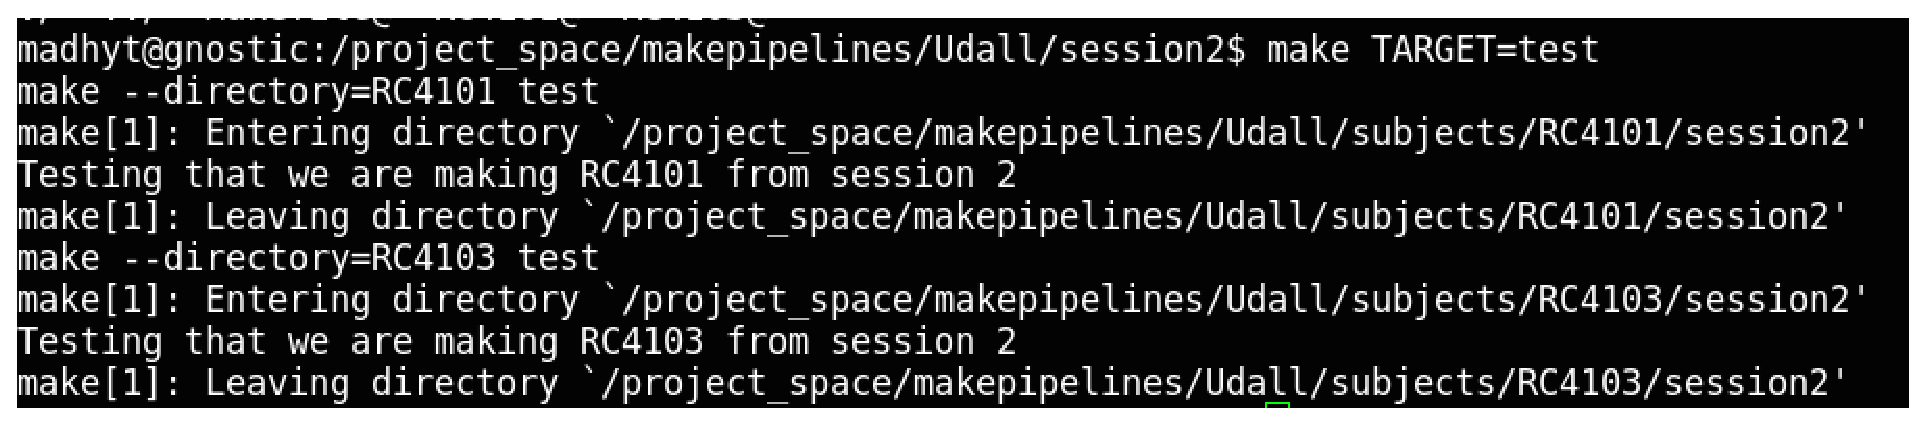
\includegraphics[width=\textwidth]{../images/make-output.eps}
	\caption{Output of recursive make}
	\label{fig:recursivemake}
\end{figure}

\section{Setting Important Variables}

\maken{} uses variables to control a lot of aspects of its own behavior. We describe only a few here; see the \href{http://www.gnu.org/software/make/manual/}{GNU Make manual} for the full list. However, it also allows you to set variables so that you can avoid unnecessary changes to makefiles when you move them to different projects. This is very important, because after going through the hassle of writing a makefile for an analysis once, we would like to reuse as much of it as possible for subsequent studies. It is reasonable to change the recipes to reflect the most appropriate scientific methods or new versions of software, but it's not fun to have to play with naming conventions, etc. We discuss some of the best practices we have found for using variables to improve portability.

\subsection{Variables that control \maken{}'s Behavior}

\subsubsection{\texttt{SHELL}}
By default the shell used by make recipes is \texttt{/bin/sh}.  This shell is one of many that you can use interactively in Linux or MacOS, but it probably is not what you are using interactively (because it lacks nice editing capabilities and is less usable than other shells). Here, we set the default shell to \texttt{/bin/bash}, the same as what we use interactively, so that we can be sure when we test something at the command line that it will work similarly in a Makefile.

\begin{make}{Setting \texttt{\$(SHELL)}}{make:shell}
	\# Set the default shell \\
	SHELL=/bin/bash \\
	export SHELL
\end{make}

Note that a \maken{} variable is accessed within \maken{} by prefixing it with a \$ sign and surrounding it with parentheses. Therefore, \texttt{SHELL} is accessed within \maken{} as \texttt{\$(SHELL)}.

\subsubsection{\texttt{TARGET}}
In the strategy that we outline for organizing makefiles and conducting subject-level analyses, we run \maken{} recursively (i.e., within the subject directories) from the session-level directory. To do this very generally, we call make from the session-level by specifying the TARGET, or what it should ``make'' within the subject directory. You do not need to do this within the subject directory itself. For example:

(in \texttt{subjects/session1})
\bashcmd{make TARGET=convert_dicoms}

(in \texttt{subjects/session1/s001})
\bashcmd{make convert_dicoms}

\subsubsection{\texttt{SUBJECTS}}
We think it makes life easier to set this variable to the list of subjects in the study (or subjects for whom data has been collected). For example, given our directory structure, when in the top level for a session, the subject identifiers can easily be found with a wildcard on the directory names. The following statement sets the variable \texttt{SUBJECTS} to be all the six-digit files in the current directory (i.e., all the subject directories.) 

\makecmd{SUBJECTS=\$(wildcard [0-9][0-9][0-9][0-9][0-9][0-9])}

\subsubsection{\texttt{subject}}
Often makefiles are intended to process a single subject. In this case, it is useful to set a subject variable to be the subject identifier.

\subsubsection{\texttt{SESSION}}
When subject data is collected at multiple time points, it is useful to set a \texttt{SESSION} variable that can be used to locate the correct subject files. 

\subsection{Other important variables}
Ultimately, when it comes time to publish, it is important to state what version of the different software packages you have used. This means that you need to make it difficult to accidentally run a job with a different version of the software. For example, consider this rule to run \texttt{DTIPrep}, a program for eddy correction, motion correction, and removal of noise from DTI images. % TO DO: cite DTIPrep

\begin{make}{Running DTIPrep in make}{make:dtiprep}
	\maker{dtiprep/\$(subject)_dwi_QCReport.txt}{dtiprep\$(subject)_dwi.nhdr} \\
	\tab DTIPrep \dd DWINrrdFile \$< -p dtiprep/default.xml \dd default \dd check \dd outputFolder dtiprep/ \\
\end{make}

Unless you take preventative measures, the version of \texttt{DTIPrep} that is used depends entirely on the caller's path. So if the version of \texttt{DTIPrep} on one machine is newer than that on another, results may differ. Alternatively, if my graduate student runs this makefile, and happens to have the newest version of DTIPrep installed in their own \texttt{bin/} directory, that is the version that will be used. This is a big problem for reproducibility.

A practical way to control for this is to specify the location of the program (if that conveys version information) as in \autoref{make:dtiv}.

\begin{make}{Controlling software version}{make:dtiv}
	DTIPREPHOME=/usr/local/DTIPrep_1.1.1_linux64/DTIPrep \\
	
	\maker{dtiprep/\$(subject)_dwi_QCReport.txt}{dtiprep\$(subject)_dwi.nhdr} \\
	\tab \$(DTIPREPHOME)/DTIPrep \dd DWINrrdFile \$< -p dtiprep/default.xml \dd default \dd check \dd outputFolder dtiprep/ \\	
\end{make}

What about when the programs are installed in some default location, e.g. \texttt{/usr/local/bin/}, with no version information? In our installation, this occurs frequently when using other workflow scripts that express pipelines more complicated than what might reasonably be put into a makefile.

In the case of simple scripts or statically linked programs, it is fairly easy to copy them into a project-specific bin directory, giving them names that indicate their versions. If you cannot do this, you need to check the version (if the program is kind enough to provide an option that will provide the version) or to check the date that the program was installed, to alert yourself to potential errors. It is useful to set variables for things like reference brains, templates, and so forth. 

\subsection{Variable overrides}
It is probably a good idea not to edit a makefile too much once it works. But sometimes, it is useful to reissue a command with different parameters. Target-specific variables may be specified in the makefile and overridden on the command line. In the example below, the default flags for FSL \texttt{bet} are specified as \texttt{-f .4 -B }.

\begin{make}{Specifying BET flags in make}{make:betflags}
	BETFLAGS = -f .4 -B \\
	\maker{\%skstrip.nii.gz}{\%flair.nii.gz} \\
	\tab bet \$< \$@ \$(BETFLAGS) \\
\end{make}

However, these can be overriden from the command line as follows:

\makecmd{make BETFLAGS='-f .4 -R'} 

\subsection{Suggested targets}
These suggestions come from experience building pipelines. Having conventions, so that similarly named targets do similar kinds of things across different neuroimaging workflows, is rather helpful and comforting, especially when you spend a lot of time going between modalities and tools.

We propose splitting functions into multiple makefiles that can then be called from a common makefile. It is helpful to avoid overruling target names for common targets. See \nameref{example:testsubject} for an example of how this is done in practice.

\texttt{all}

This is the default, the first target in the file. Nothing in this target should require human intervention. \\

\texttt{help} 

We use a \href{http://www.cmcrossroads.com/article/self-documenting-makefiles}{help system described by John Graham-Cumming}, described in \nameref{sec:practicum4}, to document makefiles. You can approach any makefile by typing \texttt{make} and get a list of documented targets and their line numbers. From the programmer's perspective, it is easy to add documentation to a target, because the call to print help and the target are located right next to each other. \\

\texttt{clean} 

Typically this target is used to remove all generated files (e.g., .o, dependency lists) and clean up the directory to its original state so that one can type "make" again and regenerate. So the idea is that ``\texttt{make clean}'' will clear the decks to allow you to restart the pipeline from scratch. This is particularly useful if you have accidentally altered some files and would like to make sure that you know exactly what processing has occurred. \\

\texttt{mostlyclean} (or \texttt{archive})

This is the same as clean, but does not remove things that are a pain to recreate (e.g., involve hand checking, or time-consuming analysis) or are critical results for publication. We use this because we are perpetually short of disk space, and this helps to clean up.  \\



\subsubsection{.PHONY}
.PHONY (the period in front is necessary) is a special target used to tell \maken{} which targets are not real files. For example, common targets are \texttt{all} (to make everything) and \texttt{clean} (to remove everything). If you create a file named ``all'' or ``clean'' in the directory with the makefile, suddenly \maken{} will see that the target file ``all'' exists, and will not do anything if it is newer than its dependencies.

To stop this rather unexpected behavior, list targets that are not real files as .PHONY:

\makecmd{.PHONY: all clean anything_else_that_is_not_a_file}

\subsubsection{.SECONDARY}
This target is used to define files that are created as intermediate products by implicit rules, but that you don't want deleted. This is critically important - perhaps a good philosophy is to define here all the files that are a pain to recreate. See \nameref{practicum1} for a lesson on secondary targets. 

\subsubsection{.INTERMEDIATE}
This target allows you to specify files that can be automatically deleted after the final targets are created. For example, during resting state preprocessing (\nameref{example:restingstate}) you create many intermediate files during the process (e.g., the output of motion correction, despiking). These are useful to check for QA purposes but in the end you may not want to keep them. Specifying them as intermediate targets will delete them after completion of the pipeline.

If you specify targets as intermediate, but you leave \texttt{.SECONDARY} blank, intermediates are treated as secondary and are not deleted automatically.  However, if you delete them (e.g., in a \texttt{clean} target), they will not be recreated when you run make again so long as the targets depending on them already exist.



